\section{Shuffle Optimization}
\label{opt}
This section presents detailed methodologies to achieve shuffle optimization. 
{\color{black}
Firstly, we discuss the reason causes shuffle overhead in the DAG frameworks.
In the following subsection, we propose a shuffle data management system to decouple shuffle from execution. 
And we propose the pre-scheduling and pre-fetching to hide shuffle overhead in multi-round map tasks.
Furthermore, two heuristic algorithms (Algorithm \ref{hminheap}, \ref{mhminheap}) are used to improve the accuracy of prediction in the pre-scheduling.
}

% The out-of-framework shuffle data management is used to decouple shuffle from execution and provide a cross-framework optimization. 
% Two heuristic algorithms (Algorithm \ref{hminheap}, \ref{mhminheap}) and a co-scheduler is used to achieve shuffle data pre-fetching without launching tasks.


\begin{figure}
	\centering
	% \begin{subfigure}[b]{0.31\linewidth}
		% 	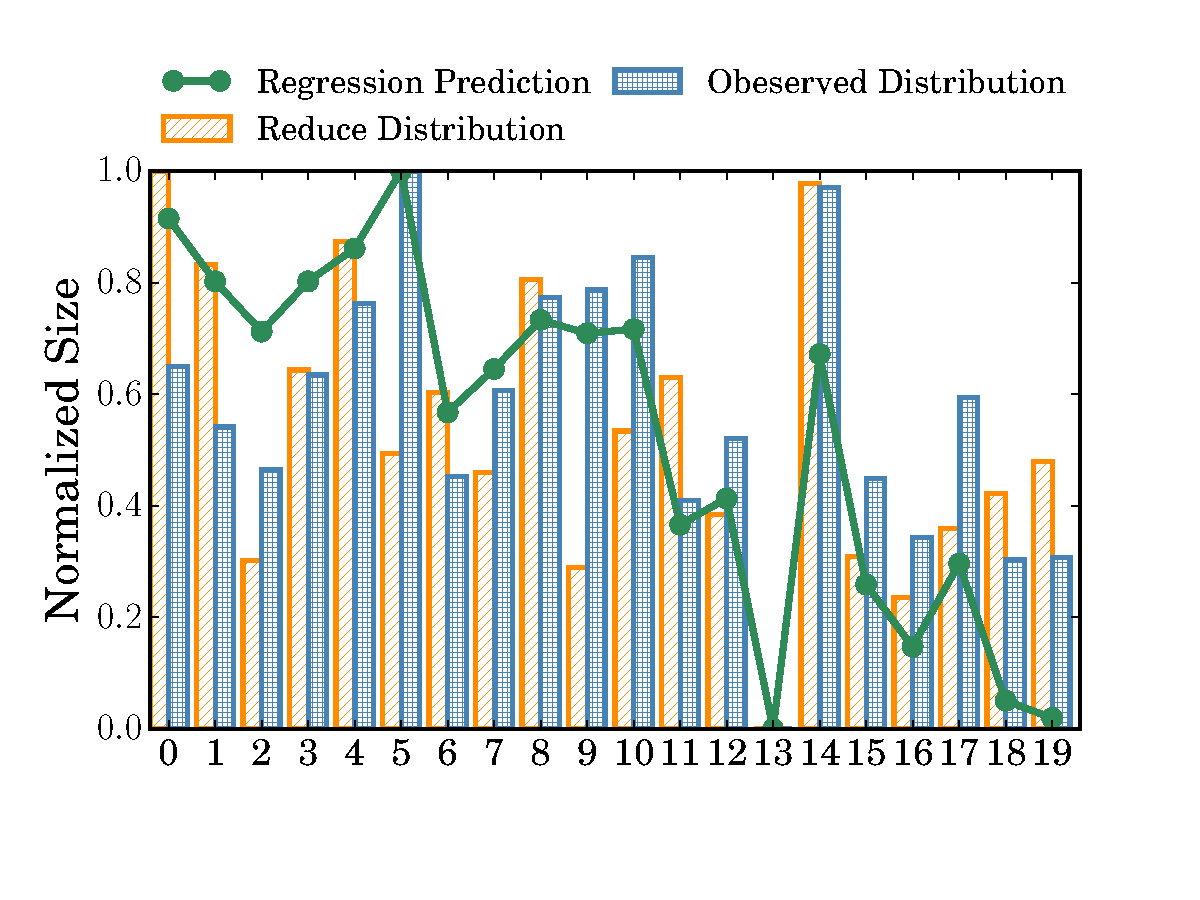
\includegraphics[width=\linewidth]{fig/hash_pre}
		% 	\caption{Linear Regression Prediction of Hash Partitioner\newline}
		% 	\label{fig:hash_pre}
	% \end{subfigure}
	\begin{subfigure}{0.75\linewidth}
		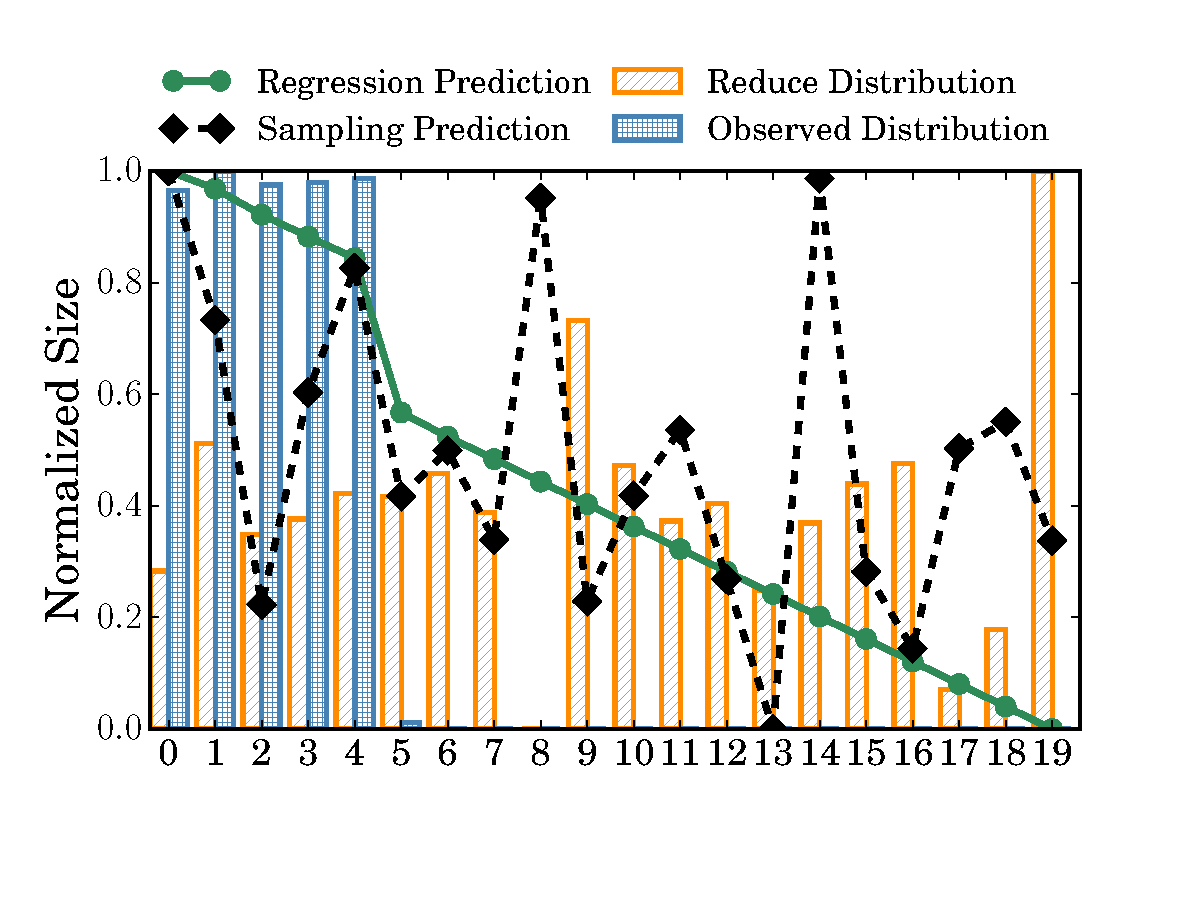
\includegraphics[width=\linewidth]{fig/range_pre_sample}
		\caption{Linear Regression and Sampling Prediction of Range Partitioner}
		\label{fig:range_pre_sample}
		% \vspace{1em}
	\end{subfigure}
	\begin{subfigure}{0.75\linewidth}
		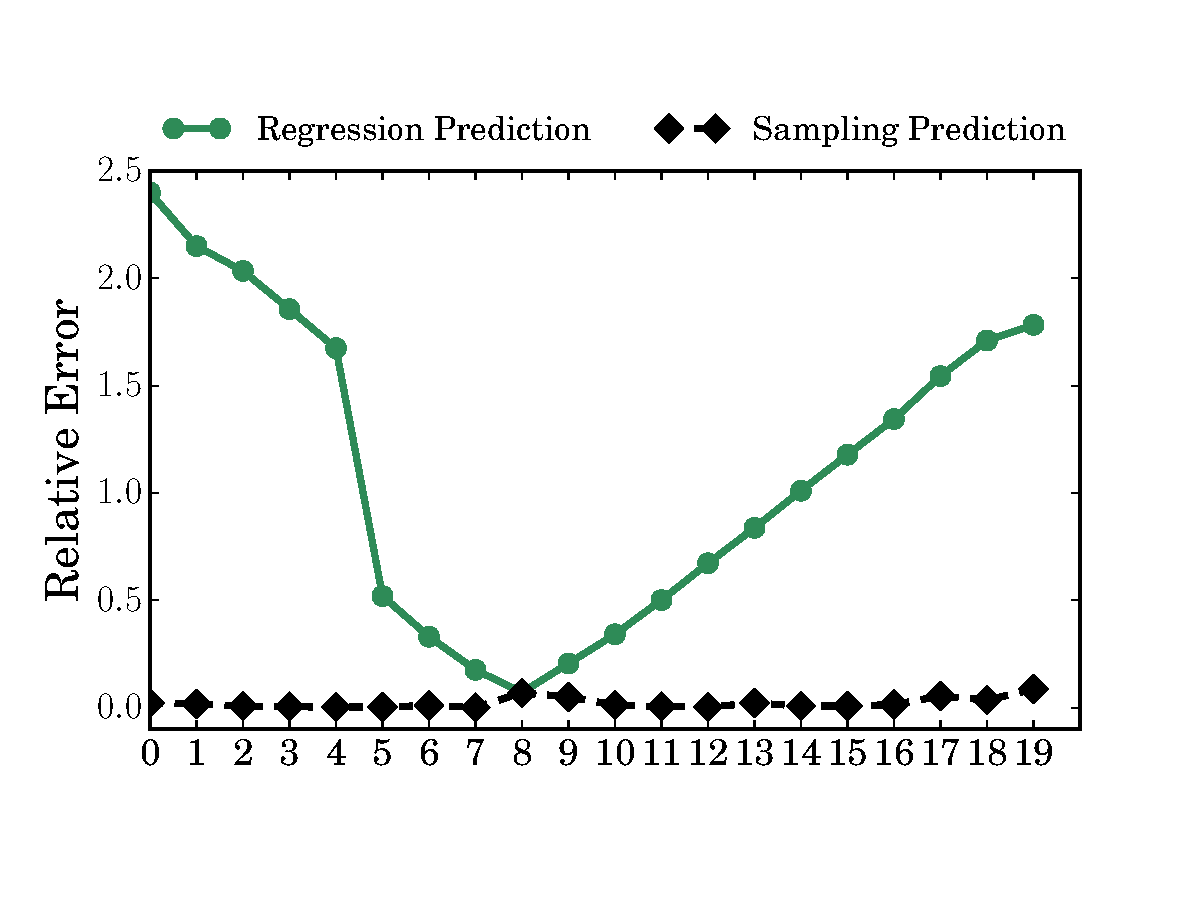
\includegraphics[width=\linewidth]{fig/prediction_relative_error}
		\caption{Prediction Relative Error of Range Partitioner\newline}
		\label{fig:prediction_relative_error}
	\end{subfigure}
	\caption{Reduction Distribution Prediction}
	\label{fig:dis}
	% \vspace{-1em}
\end{figure}
\begin{figure}
	\centering
	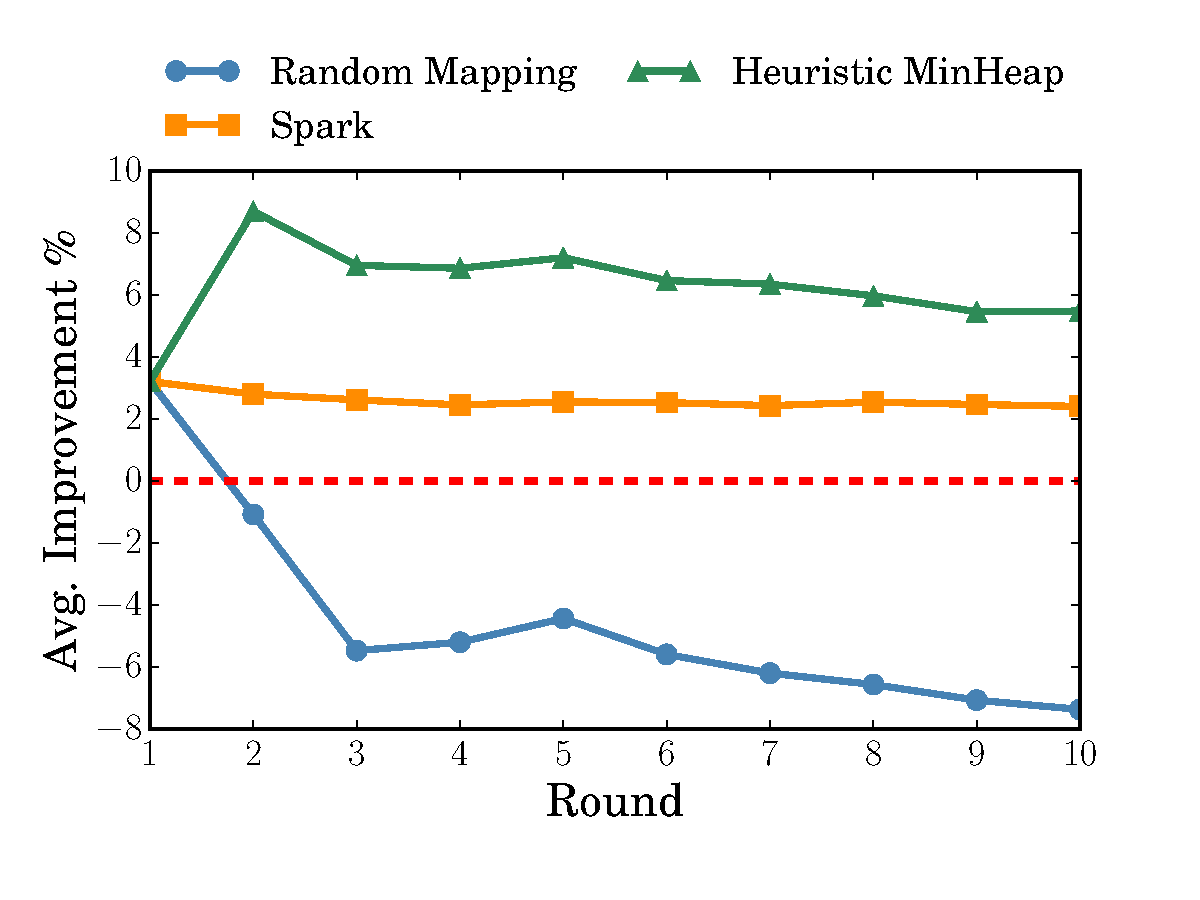
\includegraphics[width=0.75\linewidth]{fig/sim} % second figure itself
	\caption{Stage Completion Time Improvement of OpenCloud Trace}
	\label{fig:sim}
\end{figure}

{\color{black}
\subsection{Observations}\label{observation}
% DAG - shuffle - couple \& dependency - overhead in job - formula - how to optimize? - decouple \& pre-fetch - memory

In distributed computing, we use shuffle to do all-to-all data transfer among the nodes.
For a clear illustration, we divide a computing job into three phases: map, shuffle, and reduce.
In most of the DAG frameworks, including Spark, Hadoop MapReduce, and Tez, shuffle phase is coupled with reduce phase which means that shuffle data transfer and reduce computing start simultaneously.
On the reduce side, shuffle introduces an explicit overhead during shuffle read.
% Because the reduce computing depends on the shuffle results, the waiting for the shuffle data causes the overhead.
% because all reduce tasks start shuffle read simultaneously, 
Furthermore, the synchronized shuffle read causes a burst of network traffic and further enlarges the overhead.

% To better illustrate the shuffle optimization, we use this formula to represent the job completion time: \(T_{Job}=T_{Map}+T_{Reduce}+T_{overhead}\). \(T_{Map}\) represents the completion time of map phase and \(T_{Reduce}\) represents the reduce phase time without being affected by the coupled shuffle phase. 
% We use \(T_{overhead}\) to represent the above-mentioned overhead caused by shuffle.
% In the following subsections, we introduce how we decouple the shuffle and use pre-fetching and memory cache to mitigate the overhead.
To mitigate the shuffle overhead, we propose an optimization to overlap the shuffle data transfer in multi-round map tasks, and use memory to cache the shuffle data. To achieve this optimization:
\begin{itemize}
	\item Shuffle phase should be decoupled from reduce phase to achieve a better scheduling scheme.
	\item Reduce tasks should be pre-scheduled in map phase to achieve shuffle data pre-fetching.
\end{itemize}
% In Section \ref{model}, we also propose a performance model called the FRQ to model the optimization.
}

\subsection{Decouple Shuffle from Execution}
{\color{black}
To decouple the shuffle from reduce tasks, we propose a shuffle data management system called SCache to take over all shuffle data from the DAG frameworks.
SCache provides two APIs named $putBlock$ and $getBlock$ to manage the shuffle data.
On the map side, after shuffle data blocks are produced, the map task uses $putBlock$ to transfer the data blocks to SCache.
%  instead of keeping them on local storage.
Inside the $putBlock$, SCache uses memory copy to move the shuffle data blocks to SCache's reserved memory and release the slot immediately.
After getting the shuffle data, SCache starts to shuffling data immediately.
% SCache gets the shuffle data as soon as the end of a map task's execution and starts to shuffling data immediately.
% SCache leverages the property of multi-round tasks to 
On the reduce side, due to the shuffle data pre-fetching of SCache, the reduce task use $getBlock$ to get the shuffle data from SCache.

SCache caches the shuffle data on the memory instead of storing on disk \edited{like} Spark or Hadoop MapReduce.
In this aspect, SCache optimizes the time of shuffle read and shuffle write since memory gets better I/O performance.
}
% To achieve the decoupling of map tasks and reduce tasks, the original shuffle write and read implementation in the current frameworks should be modified to apply the API of SCache.
% To prevent the release of a slot being blocked by shuffle write,  
% SCache provides a disk-write-like API named $putBlock$ to handle the storage of partitioned shuffle data blocks produced by a map task.
% Inside the $putBlock$, SCache uses memory copy to move the shuffle data blocks to SCache's reserved memory and release the slot immediately.
% Inside the $putBlock$, SCache uses memory copy to move the shuffle data blocks out of map tasks and store them in the reserved memory.
% After the memory copy, the slot will be released immediately.

% From the perspective of reduce task, SCache provides an API named $getBlock$ to replace the original implementation of shuffle read. 
% With the precondition of shuffle data pre-fetching, 
% the $getBlock$ leverages the memory copy to fetch the shuffle data from the local memory of SCache.

% \subsection{Pre-scheduling with Application Context}
{\color{black}
\subsection{Pre-scheduling and Pre-fetching Shuffle Data}
% multi-round -> how to optimize? -> pre-schedule -> pre-fetch -> formula
The pre-scheduling and pre-fetching are the most critical aspects of the optimization.
% Multi-round tasks execution is used to gain better parallelism in most of DAG frameworks. For example, Spark recommends 2-3 tasks per CPU core in tasks configuration.
% Since shuffle data is available as soon as the map task finished, and the network is idle in map phases, 
SCache starts pre-fetching and hides shuffle overhead into multi-round map tasks.
However, the shuffle data cannot be pre-fetched without the awareness of task-node mapping.

To optimize shuffle phase, we propose a co-scheduling scheme with two heuristic algorithms (Algorithm \ref{hminheap}, \ref{mhminheap}). 
The DAG frameworks follow the co-scheduler to start reduce tasks.
}
% The pre-scheduling and pre-fetching are the most critical aspects of the optimization. 
% The task-node mapping is not determined until tasks are scheduled by the scheduler of DAG framework. 
% Once the tasks are scheduled, the slots will be occupied to launch them. 
% And the shuffle data cannot be pre-fetched without the awareness of task-node mapping.
% We propose a co-scheduling scheme with two heuristic algorithms (Algorithm \ref{hminheap}, \ref{mhminheap}). 
% That is, the task-node mapping is established a priori, and then it is enforced by the co-scheduler when the DAG framework starts task scheduling. 

% \subsubsection{Random Mapping Problem}\label{randomassign}
% {\color{black}
% % Mapping tasks to nodes randomly and evenly is the simplest pre-scheduling way.
% To evaluate the performance of scheduling strategies, we use traces from OpenCloud\footnote{\label{fn:trace}http://ftp.pdl.cmu.edu/pub/datasets/hla/dataset.html} for the simulation.
% As shown in Figure \ref{fig:sim}, the baseline (i.e., red dotted line) is the stage completion time with Spark FIFO scheduling algorithm. 
% We run the simulation under three scheduling schemes: random mapping, Spark FIFO, and our heuristic MinHeap.
% The performance of random mapping drops as the round number grows. 
% This is because the data skew commonly exists in data-parallel computing \cite{skewtune}. 
% Several heavy tasks may be assigned to the same node, thus slowing down the whole stage. 
% In addition, randomly mapping also ignores the data locality between shuffle map output and reduce input, which may introduce extra network traffic in the cluster.
% }
% The simplest way of pre-scheduling is mapping tasks to nodes randomly and evenly. 
% We use traces from OpenCloud\footnote{\label{fn:trace}http://ftp.pdl.cmu.edu/pub/datasets/hla/dataset.html} for the simulation.
% In order to evaluate the effectiveness of random mapping, we use traces from OpenCloud\footnote{\label{fn:trace}http://ftp.pdl.cmu.edu/pub/datasets/hla/dataset.html} for the simulation.
% The average shuffle read time is $3.2\%$ of total reduce completion time.
% We remove the shuffle read time of each task and run the simulation under three scheduling schemes: random mapping, Spark FIFO, and our heuristic MinHeap.
% As shown in Figure \ref{fig:sim}, the baseline (i.e., red dotted line) is the stage completion time with Spark FIFO scheduling algorithm. 
% The performance of random mapping drops as the round number grows. 
% Random mapping works well when there is only one round of tasks, but the performance drops as the round number grows. 
% This is because that data skew commonly exists in data-parallel computing \cite{skewtune}. 
% Several heavy tasks may be assigned to the same node, thus slowing down the whole stage. 
% In addition, randomly assigned tasks also ignore the data locality between shuffle map output and reduce input, which may introduce extra network traffic in cluster.
	
\subsubsection{Shuffle Output Prediction}\label{shuffleprediction}
{\color{black}
% The problem of random mapping is obviously caused by application context (e.g., shuffle data size) ignorance. 
The simplest way of pre-scheduling is mapping tasks to nodes randomly and evenly.
But without considering job context, the random mapping scheduling shows poor performance due to data skew and ignoring data locality.
For the most DAG applications with random large scale input, 
the shuffle output can be predicted accurately by a linear regression model based on the observation that the ratio of map output size and input size are invariant given the same job configuration \cite{guo2017ishuffle}.
% Note that a balanced schedule decision can be made under the consideration of the size of each reduce task, and the size of a reduce task produced by one shuffle $reduceSize_i = \sum_{j=0}^{m} {BlockSize_{ji}}$, 
% where the $m$ is the number of map tasks that can be easily extracted from DAG information; 
% $BlockSize_{ji}$ represents the size of block which is produced by map $task_j$ for reduce $task_i$. 
% The final sizes of reduce tasks can be calculated by aggregating $reduceSize_i$ by reduce ID among all shuffle dependencies. 
% So the pre-scheduling can be made if the prediction of size of shuffle block is practical.
% For the most DAG applications with random large scale input, 
% the $BlockSize_{ji}$ in a particular shuffle can be predicted accurately by liner regression model (i.e., equation \ref{linearregresion}) based on observation that the ratio of map output size and input size are invariant given the same job configuration \cite{guo2017ishuffle}: 
% \begin{equation}
% \label{linearregresion}
% \begin{aligned}
% 	BlockSize_{ji} = a \times inputSize_j + b
% \end{aligned}
% \end{equation}
% The $inputSize_j$ is the input size of $j$th map task. 
% The $a$ and $b$ can be determined using the observed $inputSize_j$ and $BlockSize_{ji}$.
% Though the linear regression is stable in most scenarios, it can fail in some uncertainties introduced by sophisticated frameworks like Spark.  
However, the linear regression model can fail in some scenarios. 
For example, some customized partitions may cause large inconsistency between observed map output distribution and the final reduce input distribution. 
To illustrate the case, we present a particular spark job which uses the Spark RangePartitioner in Figure \ref{fig:range_pre_sample}. 
The observed map outputs are picked randomly. 
The job uses the Spark RangePartitioner and introduces an extremely high data skew.
Due to the extremely high data skew introduced by the partition, the linear regression model cannot fit the result well.
% The data partitioned by Spark RangePartitioner in Figure \ref{fig:range_pre_sample} results in a deviation from the linear regression model, because the RangePartitioner might introduce an extreme high data locality skew. 
% We present two particular examples with 20 tasks respectively in Figure \ref{fig:hash_pre} and Figure \ref{fig:range_pre_sample}. 
% The data in are normalized to $0-1$ because the prediction of SCache only produces the data distribution instead of the real size. 
% In Figure \ref{fig:range_pre_sample}, we use the distribution of second shuffle of Spark Terasort \cite{spark-tera} that are partitioned by Spark RangePartitioner \cite{apachespark}. 
% In Figure \ref{fig:hash_pre} and Figure \ref{fig:range_pre_sample}, we use different datasets with different partitioners, and normalize the distribution to $0-1$ to fit in one figure. 
% The observed map outputs are randomly picked. 
% With a random input and a hash partitioner in Figure \ref{fig:hash_pre}, the distribution of observed map output is close to the final reduce input distribution. 
% The prediction results also fit them well. 
% However, the data partitioned by Spark RangePartitioner in Figure \ref{fig:range_pre_sample} results in a deviation from the linear regression model, because the RangePartitioner might introduce an extreme high data locality skew. 
That is, for one reduce task, almost all of the input data are produced by a particular map task (e.g., the observed map tasks only produce data for reduce task 0-5 in Figure \ref{fig:range_pre_sample}).
The data locality skew results in a missing of other reduce tasks' data in the observed map outputs.

To solve this problem, we propose a new methodology named \textit{weighted reservoir sampling}.
SCache uses this method instead of the linear regression to predict output when using a RangePartitioner or a customized non-hash partitioner.
% we introduce another methodology, named \textit{weighted reservoir sampling}, as a substitution of linear regression. 
% Note that linear regression will be replaced only when a RangePartitioner or a customized non-hash partitioner occurs. 
For each map task, we use classic reservoir sampling to randomly pick $s \times p$ of samples, where $p$ is the number of reduce tasks and $s$ is a tunable number. 
After that, the map function is called locally to process the sampled data. 
Finally, the partitioned outputs are collected with the $InputSize_j$ as the weight of the samples.
The $inputSize_j$ is the input size of $j$th map task. 
% Note that sampling does not consume the input data of map tasks. 
% The $BlockSize_{ji}$ can be calculated by:
$BlockSize_{ji}$ represents the size of block which is produced by map $task_j$ for reduce $task_i$:
\begin{equation}
\label{equationsample}
\begin{aligned}
	BlockSize_{ji} &= {{InputSize_j \times \frac{sample_i}{s \times p}}} \\
	sample_i &= \text{number of samples for $reduce_i$}
\end{aligned}
\end{equation}
In Figure \ref{fig:range_pre_sample}, when $s$ is set to $3$, the result of sampling prediction is much better than linear regression. 
Figure \ref{fig:prediction_relative_error} further proves that the sampling prediction can provide a much more accurate result than the linear regression. 
% The classic reservoir sampling is designed for randomly choosing \textit{k} samples from \textit{n} items, where \textit{n} is either a very large or an unknown number \cite{reservoir}. 
% In Figure \ref{fig:range_pre_sample}, when $s$ is set to $3$, the result of sampling prediction is much better than linear regression. 
% The variance of the normalization between sampling prediction and reduce distribution is because the standard deviation of the prediction results is relatively small compared to the average prediction size, which is $0.0015$ in this example. 
% Figure \ref{fig:prediction_relative_error} further proves that the sampling prediction can provide precise result even in the dimension of absolute input size of reduce task. 
% On the other hand, the result of linear regression comes out with a large relative error. 
% Though the weighted reservoir sampling is precise, it also introduces extra overhead. 
% We will show the overhead evaluation of sampling in Section \ref{evaluation}.
% {\color{black}

% Figure \ref{fig:prediction_relative_error} proves that the sampling prediction can provide much more accurate result than the linear regression. 
% We will show the overhead evaluation of sampling in Section \ref{evaluation}. 
% }

}
During both predictions, the composition of each reduce partition is calculated as well. We define $prob_i$ as
\begin{equation}
\label{equationprob}
\begin{aligned}
	prob_i &= \max_{0 \leq j \leq m} \frac{BlockSize_{ji}}{reduceSize_i} \\
	m &= \text{number of map tasks}
\end{aligned}
\end{equation}
% Note that a balanced schedule decision can be made under the consideration of the size of each reduce task, and the size of a reduce task produced by one shuffle $reduceSize_i = \sum_{j=0}^{m} {BlockSize_{ji}}$, 
% where the $m$ is the number of map tasks that can be easily extracted from DAG information;
The $reduceSize_i$ represents the size of a reduce task, which is represented by $reduceSize_i = \sum_{j=0}^{m} {BlockSize_{ji}}$.
We use $prob_i$ to achieve a better data locality while performing shuffle pre-scheduling. 
% This parameter is used to achieve a better data locality while performing shuffle pre-scheduling. 

\begin{minipage}{0.95\columnwidth}
\begin{algorithm}[H]
\caption{Heuristic MinHeap Scheduling for Single Shuffle}
\label{hminheap}
	\begin{algorithmic}[1]
	\small
	\Procedure{schedule}{$m, host\_ids, p\_reduces$}
		\State $m\gets$ partition number of map tasks
		\State $R\gets$ sort $p\_reduces$ by size in non-increasing order
		\State $M\gets$ min-heap $\left\{ host\_id \rightarrow \left( \left[ reduces \right], size \right) \right\}$
		\State $idx\gets 0$
		\While{$idx <$ len$R$}
		% \Comment{Schedule reduces by MinHeap}
		\State $M\left[0\right].size \mathrel{+}= R\left[idx\right].size$
		\State $M\left[0\right].reduces.append\left(R\left[idx\right]\right)$
		\State $R\left[idx\right].assigned\_id \gets M \left[0\right].host\_id$
		\State Sift down $M\left[0\right]$ by $size$
		\State $idx\gets idx+1$
		\EndWhile
		\State $max\gets$ maximum size in $M$
		% \State Convert $M$ to mapping $\left\{ host\_id \rightarrow \left( \left[ rid\_arr \right], size \right) \right\}$
		\ForAll{$reduce$ in $R$}
		\Comment{Heuristic locality swap}
			\If{$reduce.assigned\_id \neq reduce.host\_id$}
				\State $p\gets reduce.prob$
				\State $norm\gets \left(p-1/m\right)/\left(1-1/m\right)/10$
				\State $upper\_bound \gets \left(1 + norm\right) \times max$
				\State SWAP\_TASKS$\left(M, reduce, upper\_bound\right)$
			\EndIf
		\EndFor\newline
		\Return $M$
	\EndProcedure
	\Procedure{swap\_tasks}{$M, reduce, upper\_bound$}
		\State Swap tasks between node $host\_id$ and node $assigned\_id$
		\State of $reduce$ without exceeding the $upper\_bound$
		\State of both nodes.\newline
		% \State Return if it is impossible.
		\Return
	\EndProcedure
	\end{algorithmic}
\end{algorithm}
\end{minipage}

\subsubsection{Heuristic MinHeap Scheduling}\label{h-minheap}
% As long as the input sizes of reduce tasks are available, the pre-scheduling is a classic scheduling problem without considering the data locality. 
% But ignoring the data locality can introduce extra network transfer. 
% In order to balance load while minimizing the network traffic, we present the Heuristic MinHeap Scheduling algorithm (Algorithm \ref{hminheap}).
To balance load while minimizing the network traffic, we present the \textit{Heuristic MinHeap Scheduling} algorithm (Algorithm \ref{hminheap}).
{\color{black}
% For the pre-scheduling itself (i.e., the first $while$ in Algorithm \ref{hminheap}), the algorithm maintains a min-heap to simulate the load of each node and applies the longest processing time rule (LPT)\footnote{http://www.designofapproxalgs.com/} to achieve $4/3\text{-}approximation$ optimum. 
To keep the pre-scheduling load balance, we maintain a min-heap in the first $while$ loop (i.e., line 6-11).
We use the min-heap to simulate the load of each node and apply the longest processing time rule (LPT)\footnote{http://www.designofapproxalgs.com/} to achieve $4/3\text{-}approximation$ optimum.
Spark FIFO only can achieve $2\text{-}approximation$ optimum.
}
% Since the sizes of tasks are considered while scheduling, \textit{Heuristic MinHeap Scheduling} can achieve a shorter makespan than Spark FIFO which is a $2\text{-}approximation$ optimum. 
% Simulation of OpenCloud trace in Figure \ref{fig:sim} also shows that \textit{Heuristic MinHeap Scheduling} has a better improvement (average 5.7\%) than the Spark FIFO (average 2.7\%).
After pre-scheduling, the task-node mapping will be adjusted according to the locality. 
The $SWAP\_TASKS$ will be triggered when the $host\_id$ of a task does not equal the $assigned\_id$.
Based on the $prob$, the normalized probability $norm$ is calculated as a bound of performance degradation. 
Inside the $SWAP\_TASKS$, tasks will be selected and swapped without exceeding the $upper\_bound$.
Since the algorithm only maintains a min-heap and traverses $reduce$ for swapping, the algorithm needs $O(n)$ operations. 

{\color{black}
To evaluate \textit{Heuristic MinHeap Scheduling} algorithm, we use traces from OpenCloud\footnote{\label{fn:trace}http://ftp.pdl.cmu.edu/pub/datasets/hla/dataset.html} for the simulation.
% As shown in Figure \ref{fig:sim}, the baseline (i.e., red dotted line) is the stage completion time with Spark FIFO scheduling algorithm. 
As shown in Figure \ref{fig:sim}, we run the simulation under three scheduling schemes: Random Mapping, Spark FIFO, and heuristic MinHeap.
After balancing load based on the job context (e.g. shuffle size, data locality), \textit{Heuristic MinHeap Scheduling} has a better improvement (average 5.7\%) than Spark (average 2.7\%) and Random Mapping.
%  (becomes negative after the round one).
}

\begin{minipage}{0.95\columnwidth}
	\begin{algorithm}[H]
	\caption{Accumulated Heuristic Scheduling for Multi-Shuffles}
	\label{mhminheap}
		\begin{algorithmic}[1]
		\small
		\Procedure{m\_schedule}{$m, host\_id, p\_reduces, \text{\textit{shuffles}}$}
			\State $m\gets$ partition number of map tasks
			\Comment \textit{shuffles} are the previous schedule result 
			\ForAll{$r$ in $p\_reduces$}
				\State $r.size \mathrel{+}= \text{\textit{shuffles}}\left[r.rid\right].size$
				\State $new\_prob\gets \text{\textit{shuffles}}\left[r.rid\right].size / r.size$
				\If{$new\_prob\geq r.prob$}
					\State $r.prob\gets new\_prob$
					\State $r.host\_id\gets \text{\textit{shuffles}}\left[r.rid\right].assigned\_host$
				\EndIf
			\EndFor
			\State $M\gets$ $SCHEDULE\left(m, host\_id, p\_reduces\right)$
			\ForAll{$host\_id$ in $M$}
				\Comment Re-shuffle
				\ForAll{$r$ in $M\left[host\_id\right].reduces$}
					\If{$host\neq \text{\textit{shuffles}}\left[r.rid\right].assigned\_host$}
					\State Re-shuffle data to $host$
					\State $\text{\textit{shuffles}}\left[r.rid\right].assigned\_host\gets host$
					\EndIf
				\EndFor
			\EndFor
			\Return $M$
		\EndProcedure
		\end{algorithmic}
	\end{algorithm}
\end{minipage}

\subsubsection{Cope with Multiple Shuffle Dependencies}
{\color{black}
A reduce stage can have more than one shuffle dependency in the current DAG computing frameworks.
To cope with multiple shuffle dependencies, we present the \textit{Accumulated Heuristic Scheduling} algorithm.
}
% The technique mentioned in Section \ref{shuffleprediction} can only handle an ongoing shuffle. 
% For those pending shuffles, it is impossible to predict their sizes. 
% This problem can be solved by having all map tasks of pending shuffles launched simultaneously. 
% But doing this introduces large overhead such as extra task serialization. 
% To avoid violating the optimization from framework, we present the \textit{Accumulated Heuristic Scheduling} algorithm to cope with multiple shuffle dependencies.
As illustrated in Algorithm \ref{mhminheap}, the sizes of previous \textit{shuffles} scheduled by \textit{Heuristic MinHeap Scheduling} are counted. 
When a new shuffle starts, the predicted $size$, $prob$, and $host\_id$ in $p\_reduces$ are accumulated with previous \textit{shuffles}. 
After scheduling, if the new $assigned\_id$ of a reduce task is not equal the original one, a re-shuffle will be triggered to transfer data to the new host. 
This re-shuffle is rare since the previous shuffle data contributes a huge composition (i.e., high $prob$) after the accumulation, 
which leads to a higher probability of tasks swap in $SWAP\_TASKS$. 

To traverse $reduce$ for accumulating previous $shuffle$ and re-shuffling data, the algorithm needs $O(n)$ operations.
